\section{Pipeline}
\label{sec:pipeline}

Eine schematische \"Ubersicht der in diesem Projekt eingesetzten
zweistufigen Vorhersagepipeline ist in Abbildung~\ref{fig:pipeline}
dargestellt.

Die Pipeline ist so aufgebaut, dass auf eine Bildeingabe zun\"achst
eine Bildsegmentierung angewendet wird, um den Bereich des Bildes,
welcher das Nummernschild enth\"alt, herauszutrennen.
F\"ur die Bildsegmentierung wurde ein neuronales Netz trainiert,
die Einzelheiten des Verfahrens werden in Abschnitt~\ref{sec:bildsegmentierung}
n\"aher beschrieben.

Nach der Bildsegmentierung wird auf den herausgetrennten Bereich eine
Texterkennung angewendet, um die Zeichenfolge des Nummernschildes
zu extrahieren. Dieses Verfahren wird in Abschnitt~\ref{sec:texterkennung}
beschrieben.

\begin{figure}[h]
    \centering
    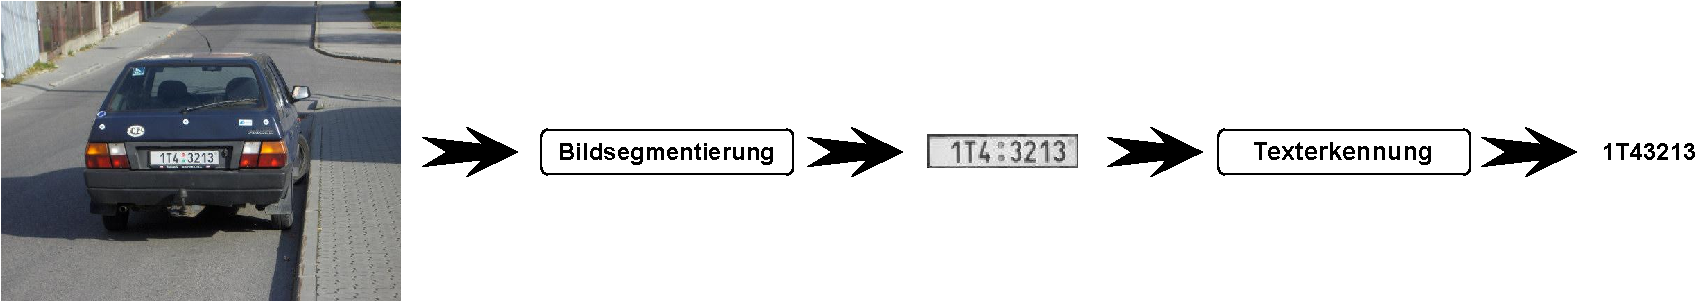
\includegraphics[width=\textwidth]{abbildungen/pipeline}
    \caption{Schematische Darstellung der zweistufigen Vorhersagepipeline.
        Zun\"achst wird das Nummernschild mithilfe von Bildsegmentierung
        extrahiert. Anschlie{\ss}end werden die Zeichen durch Texterkennung
        ausgelesen.}
    \label{fig:pipeline}
\end{figure}

\subsection{Bildsegmentierung}
\label{sec:bildsegmentierung}


\subsection{Texterkennung}
\label{sec:texterkennung}